\subsubsection{Influence of trend}
Calculated inputs showed very different results. Electricity price prediction showed an overall improvement when adding slope, skewness and volatility as input. The alternative scatter approach from Section~\ref{sec:priceExperimentThree} where previous hours are directly added as inputs for the network to calculate the relationship itself was outperformed by the direct input calculations. Skewness and volatility obtained the best result for prices with an improvement of 4\%. The results for wind power was different since only one of the calculated inputs, volatility, showed an improvement of 3,52\% compared to the same prediction without it. It was established in the analysis that both price and wind power are highly volatility and consists of different types of spikes during the year. The need for including characteristics about these spikes are discussed in Section~\ref{sec:usingStatisticalInput} but in brief it is related to the current price behaviour reflecting current market conditions\cite{yamin2004adaptive} and by including a calculation thereof we hope to add more characteristics of that particular situation \todo{find figure}. 

Using inputs that says something about the immediate past just before the 24 hours to predict can have both positive and negative results depending on what to predict as seen in our experiments. The purpose is of course to get a more precise prediction from first step and thereby achieving an overall improvement from step to step. If this is not the case and the first predicted steps are inaccurate then the error will instead elevate from step to step and make the entire 24-hour prediction more inaccurate. This is reflected in slope calculation as input for wind power in Section~\ref{sec:windPowerSlopeCalc} and seen in the comparison without it in Figure~\ref{fig:basicCurveAnalysisGraphoForDiscussion} --- this will be elaborated in coming section about step ahead prediction in Section~\ref{sec:stepAheadDiscussion}. It is noticeable that the same calculations do not apply for both even though wind power and electricity price have similar characteristics and it is therefore necessary to experiment thoroughly with the different approaches in order to find the most applicable for your dataset --- this emphasizes the discussion from the input parameters Section~\ref{sec:inputParameterDiscussion} regarding the need for describing and analysing your dataset because what worked for one dataset does not necessarily work for others if the two datasets are completely different. The calculated inputs are based on prices and productions from previous hours and because different markets are dependent on different factors \todo{find ref} it must be stated clearly what factors are used. For instance, countries with many Cooling Degree Days or Heating Degree Days, following the model in Section~\ref{sec:ElectricityDemand}, have higher consumption which greatly influence the price. The same apply for the importance of wind power in the Danish electricity market due to huge amount of wind mills which in this thesis has shown to be significant. This is not applicable for countries without the same amount of mills. The documentation is contributory factors to the potential of identifying similar markets in terms of influences. It can help identify both standard but also which calculated inputs to use for specific market conditions, e.g. if a marked is analysed to be similar to Denmark then it makes sense to use their ideas and models first. The point is again that the data analysis is considered to be so important for the ANN result that it cannot be omitted. 

\begin{figure}[H]
\centering
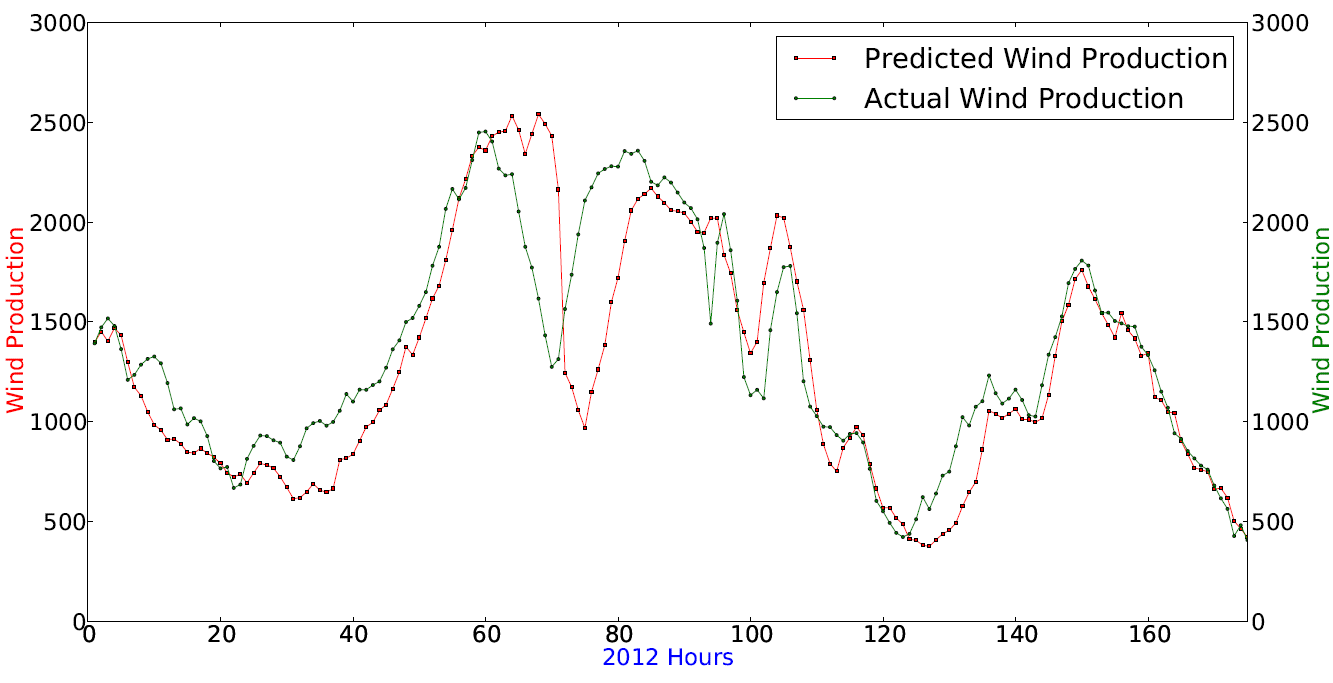
\includegraphics[width=0.99\linewidth]{billeder/curveAnalysisWindProduction.png}
\caption{Wind production prediction for 175 hours in 2012 with slope as input}
\label{fig:basicCurveAnalysisGraphoForDiscussion}
\end{figure}

It was expected to see better accuracy when applying calculated inputs to the electricity prices since it relies more heavily on previous prices and price movements as discussed in the price analysis in Section~\ref{sec:ElectricityPriceAnalysis} whereas wind power follows meteorological factors more significantly, namely wind speed. Price does not follow one parameter as close as wind power does with wind speed. This fact is apparent in the achieved MAE of 149,72 when using wind speed only to predict wind power. The experiment still verifies the improvements with an overall improvement of 19,2\% to a MAE of 121,02 as the best result. What can be concluded from the results is the potential benefit from using calculated inputs to add additional characteristics about the movements of the curve in both cases and help the generalization function of the network to approach its target better if the correct calculation inputs are used. Alternative calculations from the field of economics could potentially help improve the predictions since it could include additional features and characteristics of the curve movements. This could involve alternative ways of calculating volatility, skewness but the electricity price is also sensitive to external influences that can result in electricity price spikes\cite{singhal2011electricity}. These influences are only shortly mentioned but covers socio-cultural factors as described in Section~\ref{sec:ElectricityDemand} but also natural gas, oil, fuel prices and system loads\cite{singhal2011electricity}. This is to be explored future work. 